\subsection{Vaizdų duomenų skaitytuvo klasė}
\label{subsec:image_data_reader}

Klasė \texttt{ImageDataReader} užkrauna jau padalintas vaizdų aibes ir pritaiko vienodą \texttt{torchvision.transforms} grandinę. Skaičiavimo resursams taupyti buvo užkraunama $30\ \%$ duomenų (žr.~\ref{fig:image_data_reader_class} pav.).

\begin{figure}[H]
    \centering
    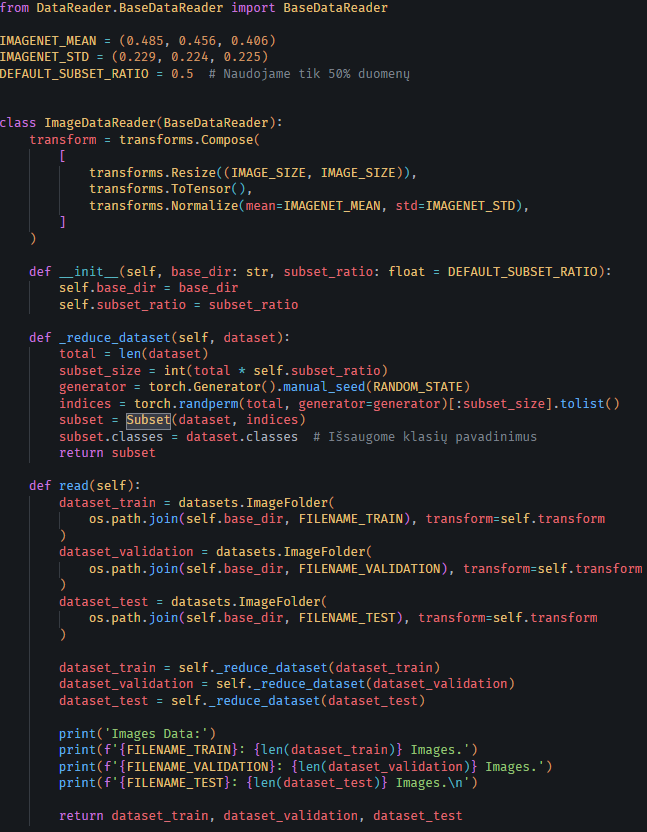
\includegraphics[width=0.85\linewidth]{3Lab/overleaf/images/ImageDataReader_Class.png}
    \caption{Vaizdų duomenų skaitytuvo klasės kodas.}
    \label{fig:image_data_reader_class}
\end{figure}

Klasės veikimo žingsniai:
\begin{enumerate}
    \item \texttt{transforms.Resize} suvienodina visus vaizdus į $64 \times 64$ raišką – tinklo įėjimo formatas turi būti pastovus.
    \item \texttt{transforms.ToTensor} konvertuoja \texttt{PIL.Image} į \texttt{torch.Tensor} ir pikselius perkelia į $[0,\,1]$ intervalą.
    \item \texttt{transforms.Normalize} standartizuoja kanalus pagal \textit{ImageNet} vidurkį ir standartinį nuokrypį, todėl tinklo svoriai pradeda mokytis stabilesnėje skaitinėje erdvėje.
    \item \texttt{\_reduce\_dataset} atsitiktinai parenka \texttt{subset\_ratio} dalį indeksų ir grąžina \texttt{torch.utils.data.Subset}. Naudojamas atskiras \texttt{torch.Generator} su \texttt{seed = 42}, todėl pošalis kiekvieną kartą yra tas pats.
    \item \texttt{read} paima visus tris \texttt{ImageFolder} aplankus (\textit{train}, \textit{validation}, \textit{test}) ir grąžina jų sumažintus pošalius.
\end{enumerate}

Klasės kodas parašytas autoriaus, naudojantis oficialia \texttt{torchvision} dokumentacija. \textit{ImageNet} statistikos reikšmės paimtos iš \texttt{torchvision} oficialaus pavyzdžio kodo.
